
\section{Results}
We pruned a four years old virtual
untrained tree (Fig.~\ref{fig:my_figure4}) by using the proposed method. The same tree was also pruned by horticulture expert and the results were compared.
The tree training teaching environment EduAPPLE~\cite{kohek_eduapple:_2015} was used for this purpose. The expert shaped the tree into two primary forms, a
pyramidal growing form (denoted as HeP -- Human expert - Pyramidal), which is similar to a Slender Spindle, and a
Flatt growing form (denoted as HeF -- Human expert - Flatt), suitable for the Fruiting Wall planting system. 
For the automated pruning, we used a cone with the height of \(3\)m and the
opening angle of \(45{^\circ}\) (denoted as DDECn -- DDE method, Conical initial shape), and a cylinder with a height of
3m and radius of 0.75 m (denoted as DDECy -- DDE method, Cylindrical initial shape). 
In both cases, we set \(s_{\mathrm{\max}}=50\). 
\begin{figure}[hbt]
    \centering
    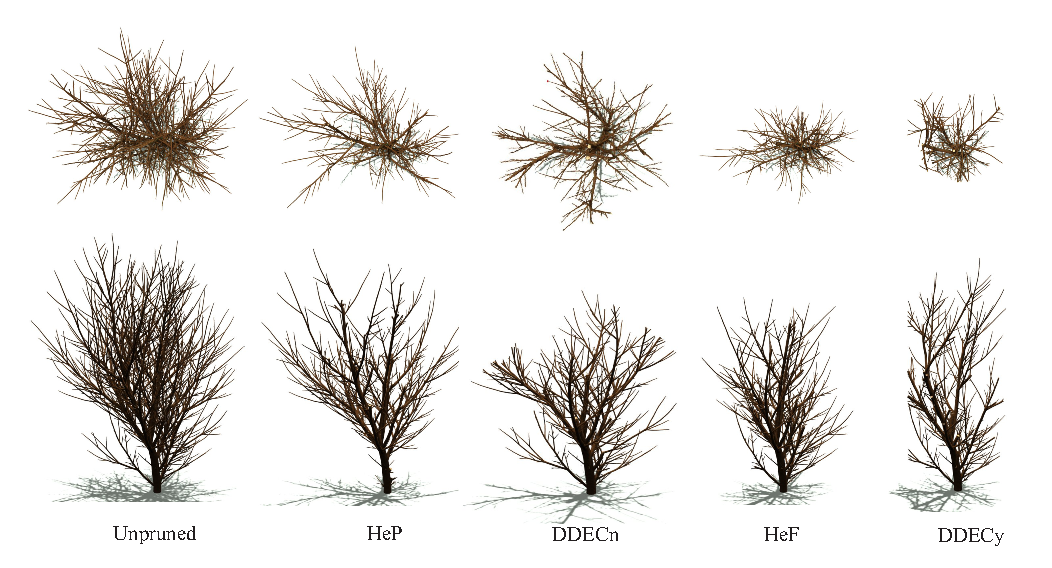
\includegraphics[width=\linewidth]{figs/Fig5.pdf}
    \caption{Comparison of pruning with the initial unpruned tree,
tree pruned by a human expert in a pyramidal shape (HeP), automated
pruning with initial cone shape (DDECn), pruning by human expert pruning
in a plat plane (HeF), automated pruning with the use of cylindrical
initial shape (DDECy).}
    \label{fig:my_figure4}
\end{figure}

\noindent\textbf{Light Distribution:} In all four cases, the light distribution inside the tree crown has
improved (see Table~\ref{tab:light}) as compared to the unpruned tree (Fig.~\ref{fig:my_figure5}) with the average increase of 168\% of buds. 
In particular, only 14.89 \% of buds receive more than 70 \% of available light in the unpruned trees, 
while in the the human-pruned tree the amount of such buds increases to 26.80 \% (HeP) and to the 22.95 \% (HeF).
The light distributions of the automated tree pruning are comparable with
that of human expert (25,93 \% for DDECn and 24.18 \% for DDECy). 
When comparing HeP to DDECn the result in the cases of human pruning is slightly better but in the case of HeF and DDECy the automated pruning achieved better result, although the difference in both casses is less than 1.3 \%.  
\begin{table}[hbt]
\label{tab:light}
\begin{center}
\begin{tabular}{ |l|c|c| } 
 \hline
 \textbf{Method} & \textbf{\% of buds receiving}                           & $\mathbf{\Delta}$ \textbf{to unpruned [\%]} \\ 
                 &  \textbf{more than 70\% of light}                       &  \\ 
 \hline
 \textbf{Unpruned}            & 14.89 & 0 \\ 
 \hline
 \textbf{Manual Expert (HeP)} & 26.80 & 180 \\ 
 \textbf{Manual Expert (HeF)} & 22.95 & 154 \\ 
  \hline
 \textbf{Automatic (DDECn)} & 25.93 & 174 \\ 
 \textbf{Automatic (DDECy)} & 24.18 & 162 \\ 
 \hline
\end{tabular}
\end{center}
\caption{The percentage of buds receiving more than 70\% of light in an unpruned tree and after manual pruning by using HeP and HeF methods and our automatic pruning by using DDECn and DDECy. The improvement in all cases is in average of 168\%. }
\end{table}

\noindent\textbf{Pruned Internodes:} The difference between the DDE and human pruning is also visible in the category of the internodes left in the tree after the pruning as shown in Table~\ref{tab:inodes}. The unpruned tree has 18,618 internodes. After manual pruning by using HeP the number decreased to 7,810 and manual pruning by using HeF decreased the number to 5,715. Automatic pruning provided smaller numbers. The DDECn algorithm pruned the tree to 5,714 and the DDECy to 4,867 nodes. The average number for manual pruning was 6,776 and for automatic 5,291.
\begin{table}[hbt]
\label{tab:inodes}
\begin{center}
\begin{tabular}{ |l|c|c| } 
 \hline
 \textbf{Method} & number of internodes on the tree  & $\Delta$ to unpruned [\%] \\ 
  \hline
 \textbf{Unpruned}            & 18,618 & 0 \\ 
 \hline
 \textbf{Manual Expert (HeP)} & 7,810 & 42 \\ 
 \textbf{Manual Expert (HeF)} & 5,715 & 31 \\ 
  \hline
 \textbf{Automatic (DDECn)} & 5,741 & 31 \\ 
 \textbf{Automatic (DDECy)} & 4,867 & 26 \\ 
 \hline
\end{tabular}
\caption{The number of internodes on the tree in an unpruned tree and the comparison to the number of internodes after manual pruning by using HeP and HeF methods and our automatic pruning by using DDECn and DDECy. The average number of internodes is 6,033 that corresponds to 32\% of nodes of the unpruned tree. }
\end{center}
\end{table}

By combining both results from Tables~\ref{tab:light} and~\ref{tab:inodes}, 
it can be concluded, that the human expert
achieved similar bud light exposure with less biomass removed,
which is desirable since the higher number of internodes with
well-illuminated buds represent the higher potential for the yield of
both increased quality and quantity. 

\begin{figure}[hbt]
    \centering
    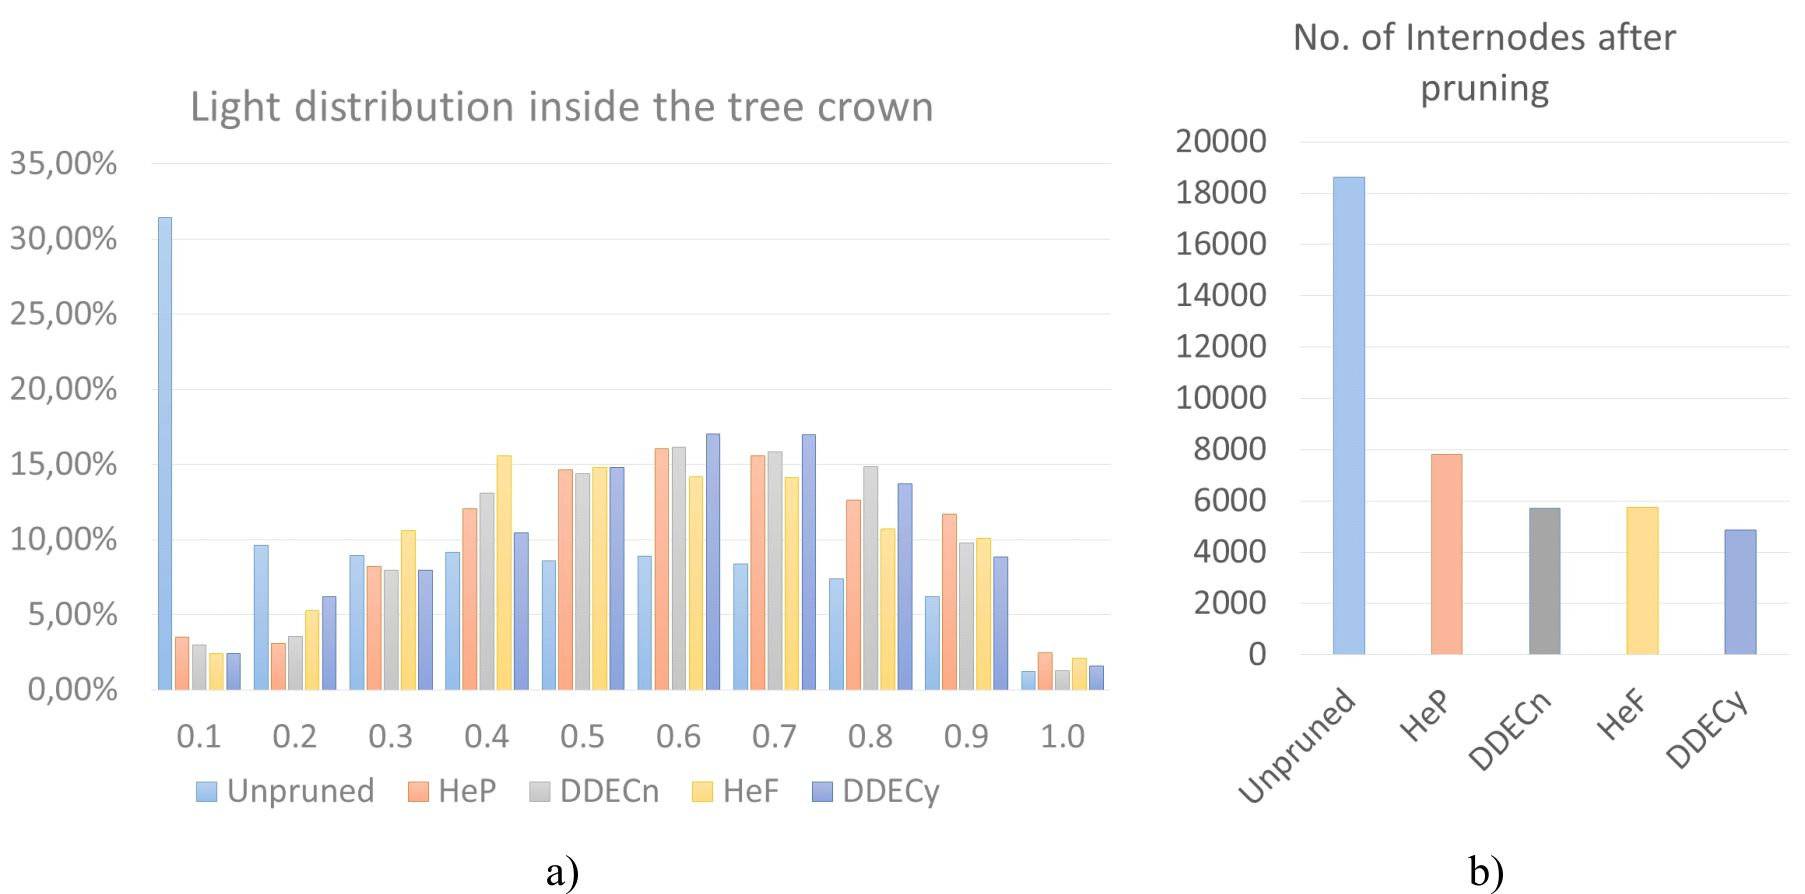
\includegraphics[width=\linewidth]{figs/image5.jpeg}
    \caption{Evaluation of tree pruning results, a) Comparison of
light distribution after the pruning by a human expert (HeP and HeF) and
automated pruning (DDECn and DDECy), b) Number of internodes left after
the pruning. A higher number of internodes, combined with higher light
exposure of buds signify better results.}
\label{fig:my_figure5}
\end{figure}

The DDECn and DDECy methods are representative of the selective pruning, where the
results of the first step represent the result of pruning by the
automatic pruning systems currently used. The difference between the
first and second step of DDECn and DDECy can be seen in Fig.~\ref{fig:my_figure6}. Visually, the trees after the second step are clearly less dense as the number of branches is drastically diminished,
while the overall height of the tree remains the same.

\begin{figure}[hbt]
    \centering
    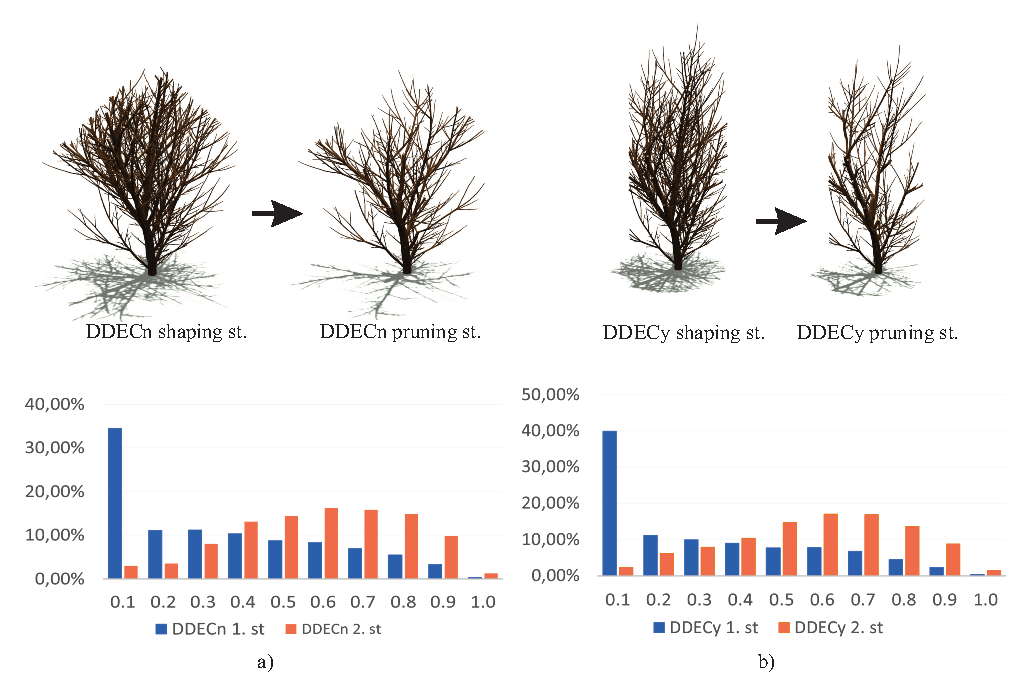
\includegraphics[width=\linewidth]{figs/Fig7.pdf}
    \caption{Tree crown light distribution after the shaping and
after the pruning step, a) DDECn method, b) DDECy method}
    \label{fig:my_figure6}
\end{figure}

\noindent\textbf{Long-term Pruning:} In another experiment, we evaluated a
long-term exposure to pruning. We were curious if the proposed automated tree pruning method is capable of tree training (i.e., getting the tree into desired growing form) without human intervention. We have
simulated a row of five trees for six consecutive years. At the
beginning of each year, the trees were pruned by the DDECn method to shape
them into the Slender Spindle growing form. The starting cone height was
1m and was linearly increased to 2.5m, which was the target height for
the trees in the following three years. The opening angle was constant
at $45^\circ$ for the experiment duration. The initial value of the parameter
\(s_{\mathrm{\max}}=20\) and was linearly increased to \(s_{\mathrm{\max}}=70\) in
the sixth year. The result of the experiment can be seen in Fig.~\ref{fig:my_figure7}.

As the tree structure becomes more complex in time, the
value of \(s_{\mathrm{\max}}\ \) should be increased. In our experiments
we observed that \(s_{\mathrm{\max}}\leq{150}\) even
for older trees provides reasonable results.
\begin{figure}[hbt]
    \centering
    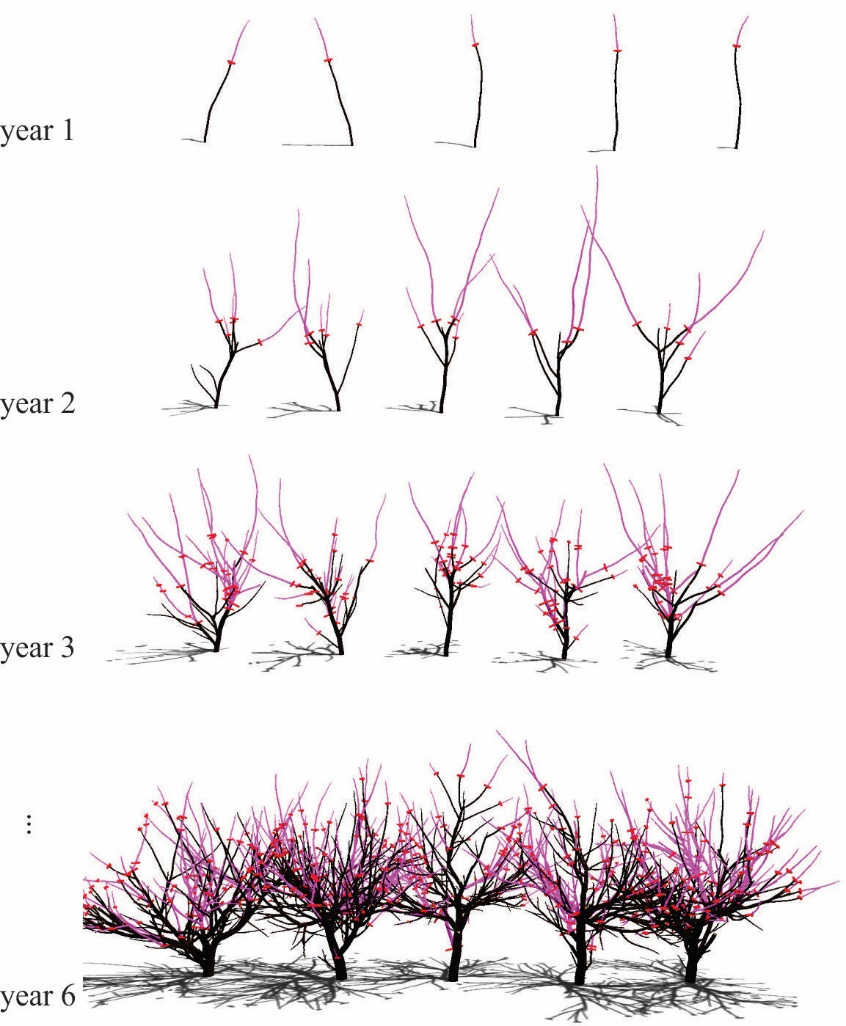
\includegraphics[width=0.75\linewidth]{figs/image7.jpeg}
    \caption{Tree training of five apple trees into a Slender
Spindle growing form for six consecutive years with the DDECn method.
The purple color denotes the branches removed at the pruning}
    \label{fig:my_figure7}
\end{figure}


